The design of the website got changed because we wanted to get a modern look of the website. As on figure login and figure signup you can see that the color and design have been changed a lot compared to figure old login (figure 3.8 i rapporten). In the previous version there wasn’t any signup ability. So this signup does only the basics like creating username, password, gender and date of birth. The color black was chosen for the background and it blends good with blue and white. the color black and white according to figure \ref{Colors}, on page \pageref{Colors}, it gives an neutrality feeling and the color blue gives calm feeling. According to empower-yourself-with-color-psychology.com \cite{EmpowerColor}, the meaning of the color is,  the color black is the secretive and the unknown, and creating an air of mystery. the color white is the color of perfection. The color blue is the color of trust and peace. The color black, white and blue is the basic colors for the website.


\begin{figure}[H]
\centering
\begin{subfigure}{.5\textwidth}
  \centering
  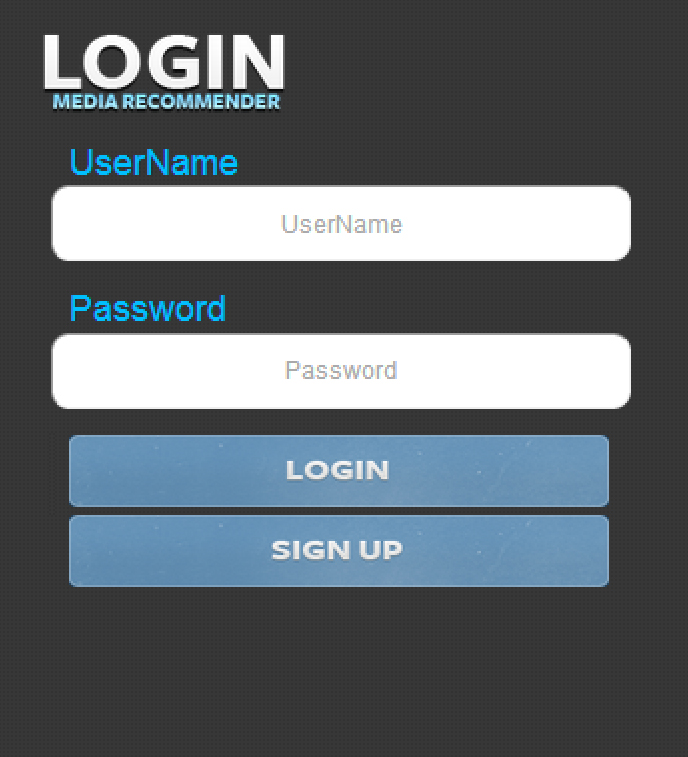
\includegraphics[width=.9\linewidth]{Images/new-login.jpg}
  \caption{Login}
  \label{fig:new-login}
\end{subfigure}%
\begin{subfigure}{.5\textwidth}
  \centering
  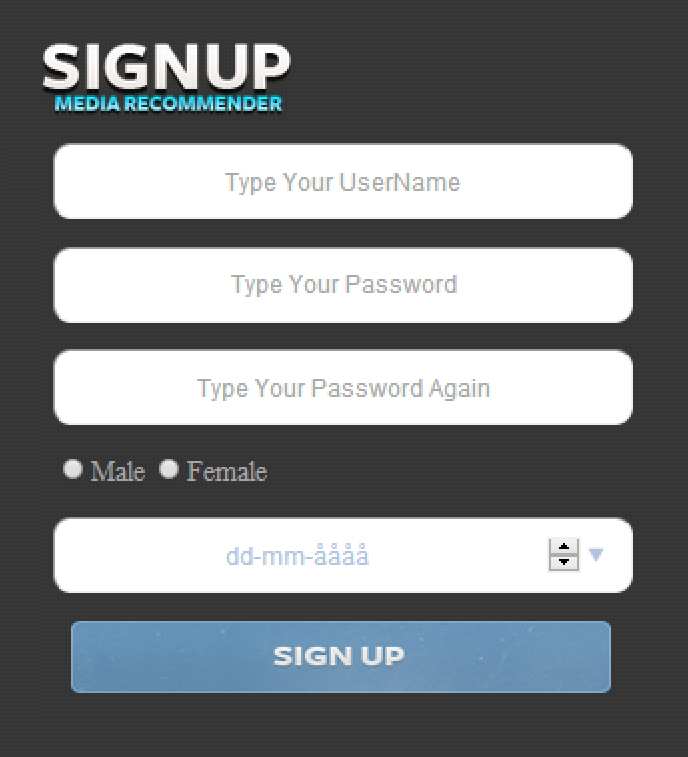
\includegraphics[width=.9\linewidth]{Images/new-signup.jpg}
  \caption{Signup}
  \label{fig:new-signup}
\end{subfigure}
\caption{Redesign of Login and Signup}
\label{fig:login-signup}
\end{figure}



After creating an user and being logged in to the website you’ll be directed to the frontpage. Compared to the old design of the website figure \ref{CurrSite}, on page \pageref{CurrSite}, there have been added search bar and an ability to specify which media and a rating ability. On the right side of figure \ref{new-frontpage} you will be able to see that movies, games and books have been combined into one button called recommendation compared to the old design figure \ref{CurrSite}. The recommendation button is chosen to be red according to figure \ref{Colors} it gives a hot feeling like what’s hot, and according to empower-yourself-with-color-psychology.com it means that you are ready to take action. 
If you rate and add a media it will give you a notification saying: “Added to your medialist”, so the user will know where his/her media will be added to.

\begin{figure}[H]
\centering
\begin{subfigure}{.5\textwidth}
  \centering
  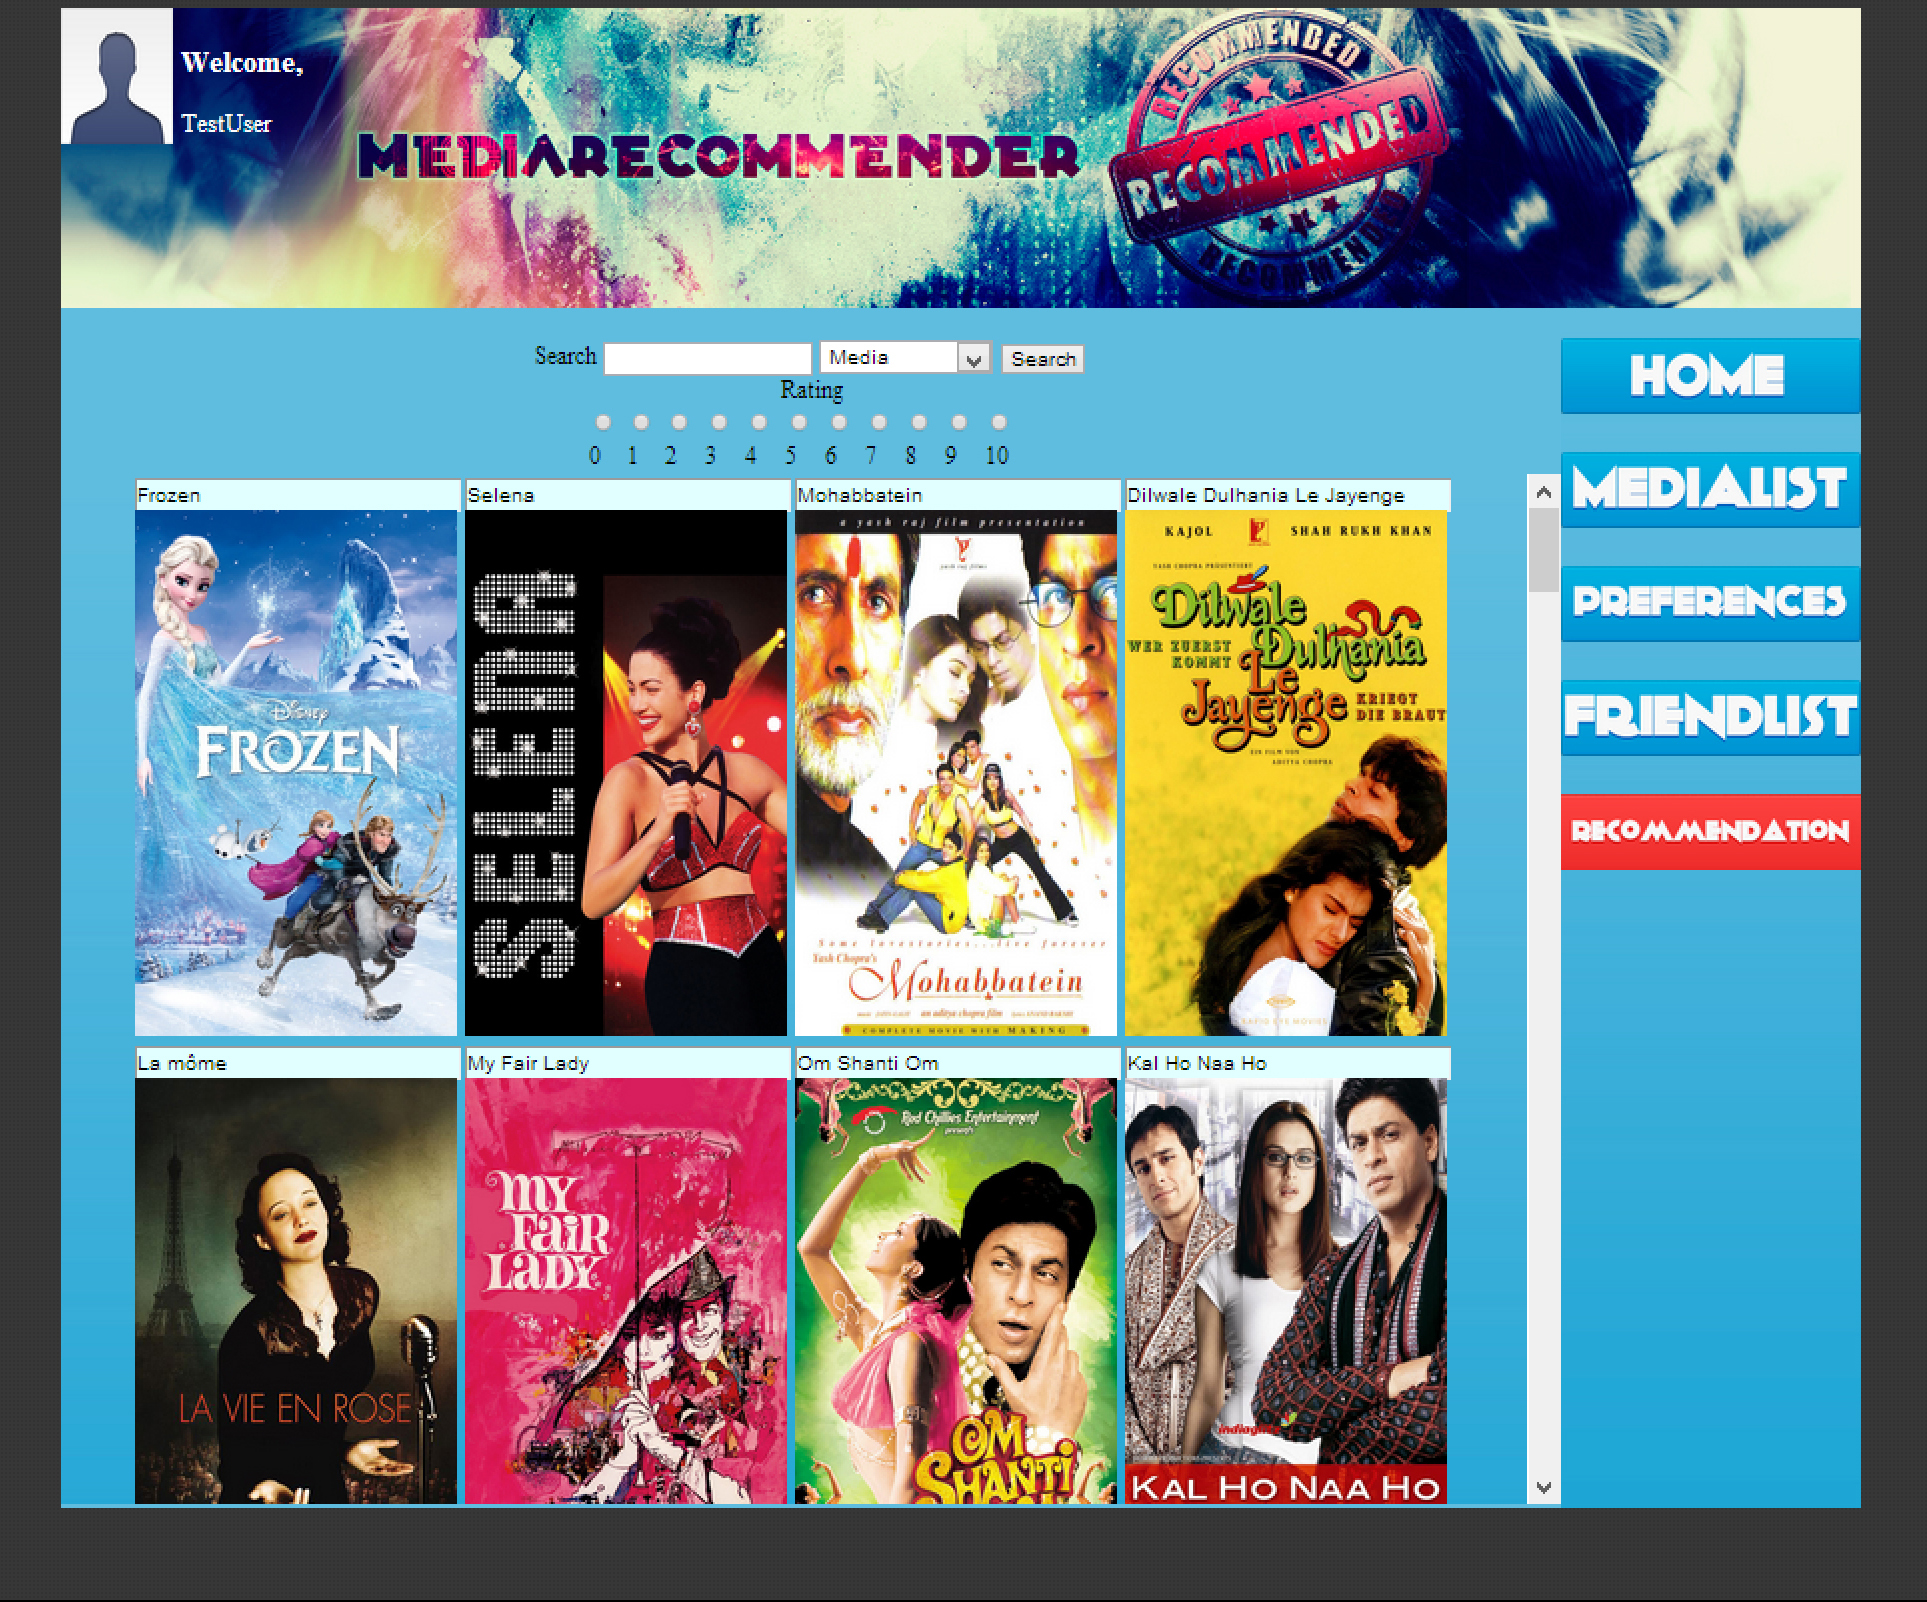
\includegraphics[width=.9\linewidth]{Images/new-home.jpg}
  \caption{Frontpage}
  \label{fig:new-frontpage}
\end{subfigure}%
\begin{subfigure}{.5\textwidth}
  \centering
  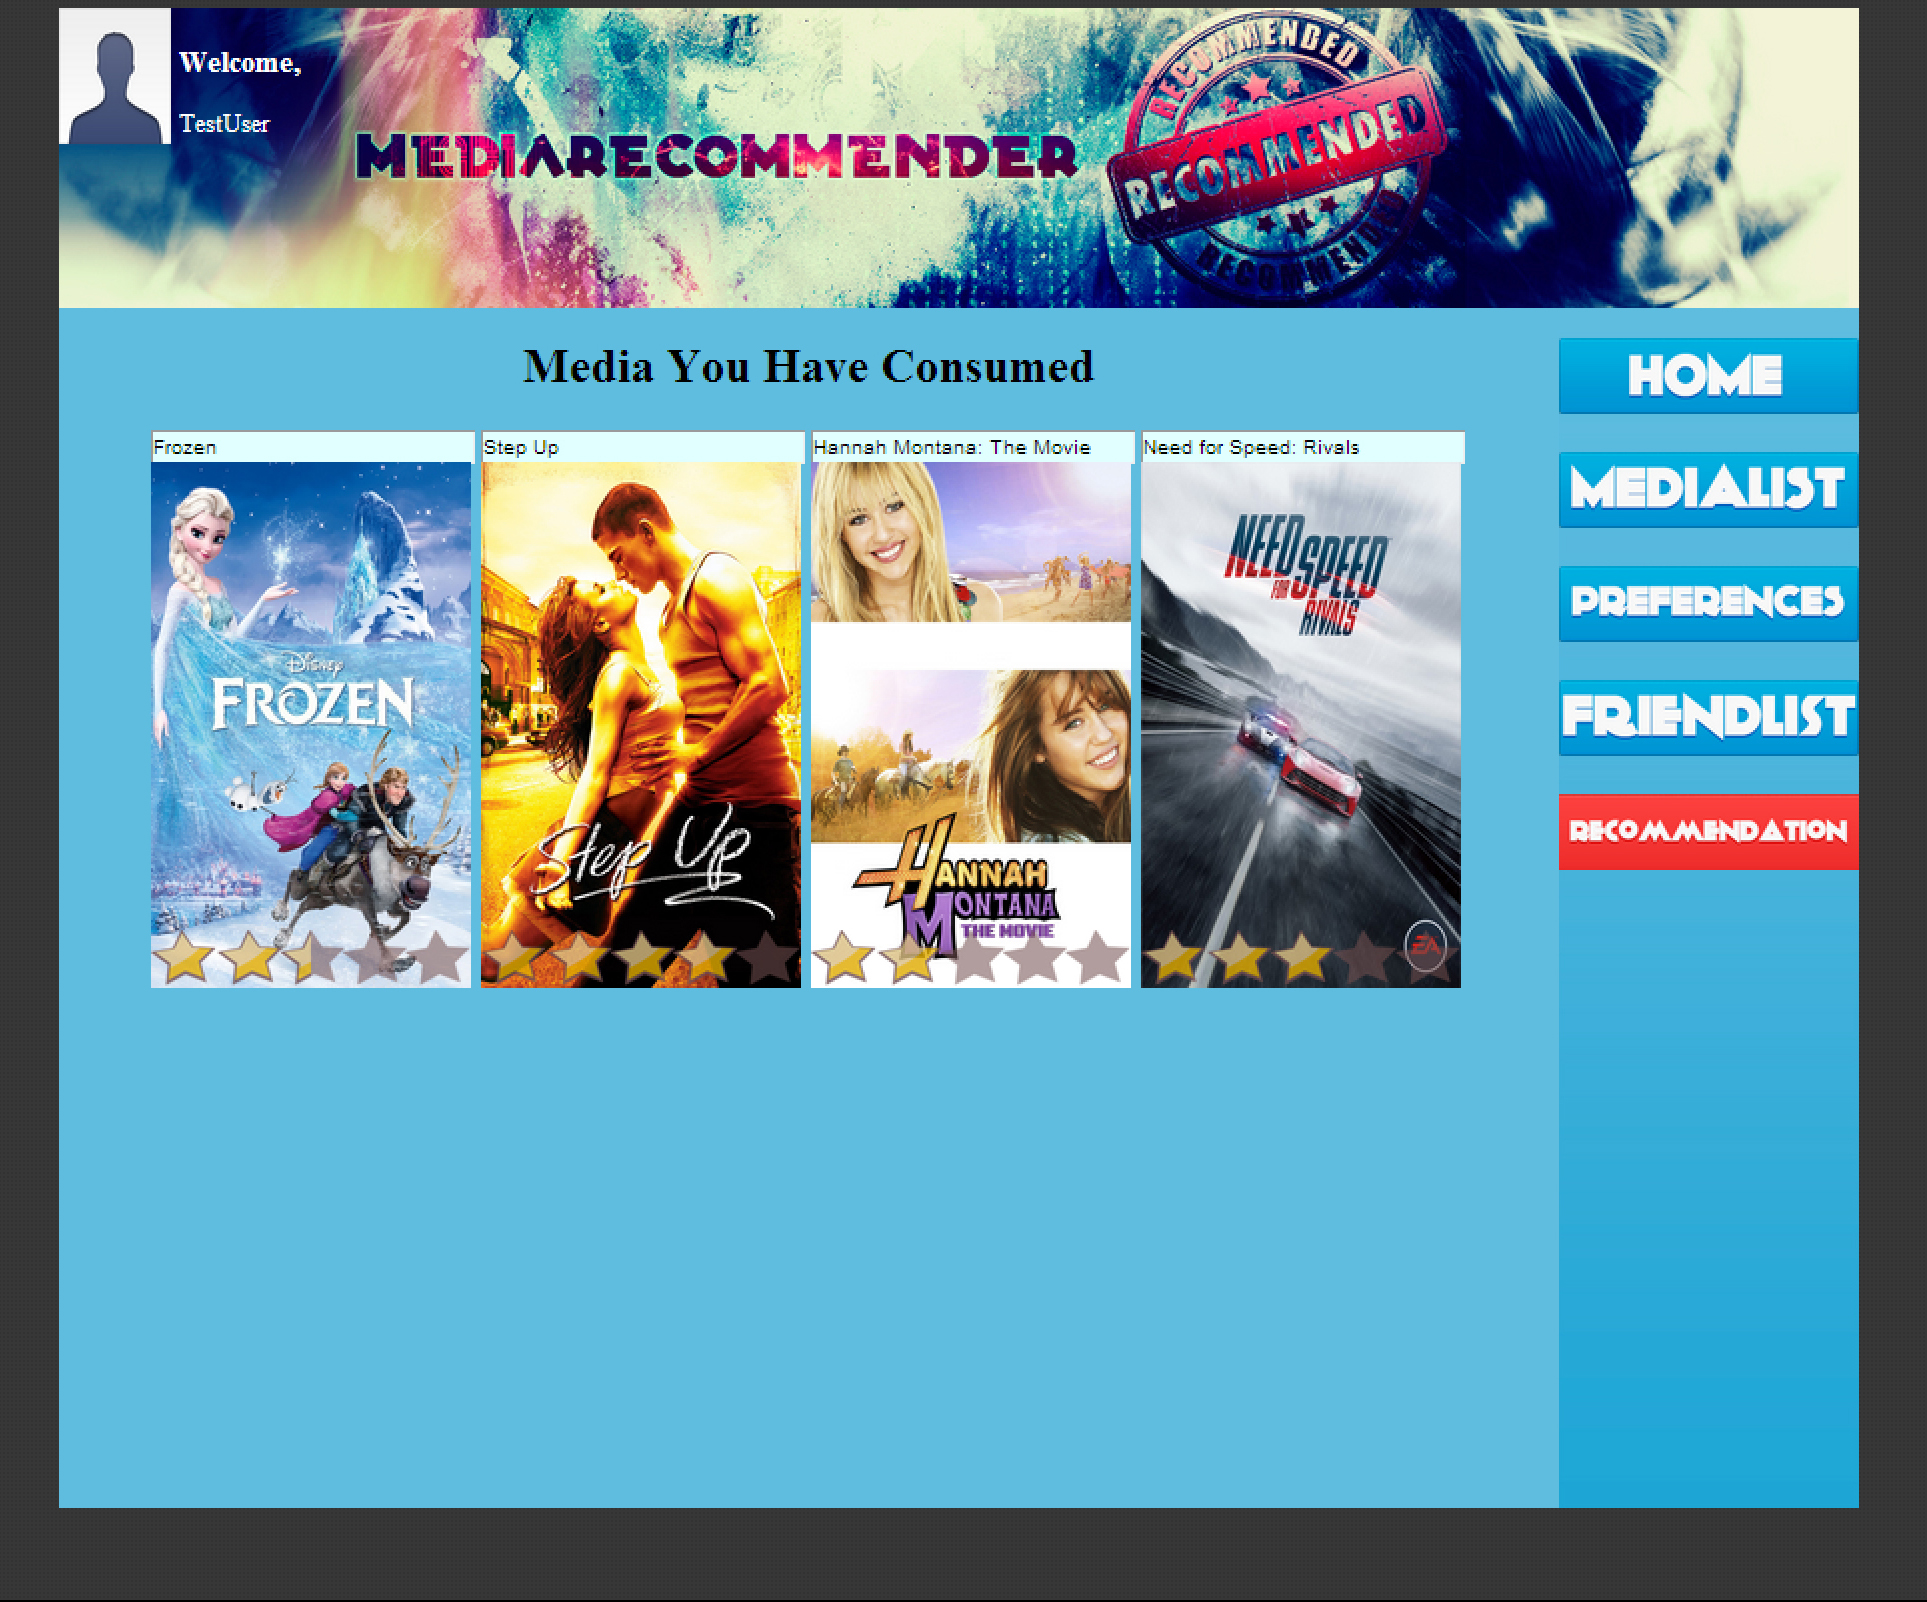
\includegraphics[width=.9\linewidth]{Images/new-medialist.jpg}
  \caption{Medialist}
  \label{fig:new-medialist}
\end{subfigure}
\caption{Redesign of frontpage and medialist}
\label{fig:front-media}
\end{figure}

On the medialist, figure \ref{fig:new-medialist} page you will see all the medias you have added to the medialist and your rating will be shown on the media cover. If you click on the media there will be shown a confirmation notification saying: “Are you sure you want to remove this media?”. Whether the user accept or not the media will be removed from the users medialist.

On the preference page is where all the genres. The user can specify what’s he/she is into. This will affect the output of the recommendation.

On the recommendation page is where the user gets his/her recommendation done by the collaborative and content based algorithms. The output of the recommendation is compared with your medialist and all other users medialist.

The design have some kind colors, which again are black, white, blue and red, to make the user feel more comfortable. The design of the website is simple that makes it easy for the user to understand since the design is a typical layout for a website.
